% iaus2esa.tex -- sample pages for Proceedings IAU Symposium document class
% (based on v1.0 cca2esam.tex)
% v1.04 released 17 May 2004 by TechBooks
%% small changes and additions made by KAvdH/IAU 4 June 2004
% Copyright (2004) International Astronomical Union

\NeedsTeXFormat{LaTeX2e}

\documentclass{iau_FM}
\usepackage{amsmath}
\usepackage{graphicx}
\usepackage{multirow}
\usepackage{natbib}
\usepackage{journals}
\usepackage{hyperref} 

\bibliographystyle{aasjournal}

\title[chapter:hardware] {Real-time RFI Excision Techniques and their limitations}
\author[Buch, Gunaratne, Hellbourg, Viou and Winkel]   %% give here short author list %%
% author list -- decide on ordering later
{
 Kaushal D. Buch$^1$
 \and Thushara Gunaratne$^2$
 \and Gregory Hellbourg$^3$
 \and Cedric Viou$^4$
 \and Benjamin Winkel$^2$
}

\affiliation{
% remove email addresses if you do not want this published
$^1$ Giant Metrewave Radio Telescope, NCRA-TIFR, Pune, India \\ email: {\tt kdbuch@gmrt.ncra.tifr.res.in}\\[\affilskip]
$^2$ Herzberg Astronomy and Astrophysics Research Center, National Research Council Canada \\ email: {\tt Thushara.Gunaratne@nrc-cnrc.gc.ca} \\[\affilskip]
$^3$ \\[\affilskip]
$^4$ ORN, Observatoire de Paris, Université PSL, Univ Orléans, CNRS, 18330 Nançay, France \\ email: {\tt Cedric.Viou@obs-nancay.fr} \\[\affilskip]
$^5$ \\[\affilskip]
}
\begin{document}

\maketitle

\begin{abstract}
Abstract
\keywords{Keyword1, keyword2, keyword3, etc.}
%% add here a maximum of 10 keywords, to be taken form the file <Keywords.txt>
\end{abstract}


\section{Introduction}
\label{section:hardware: introduction}

%\textbf{Benjamin: I think, a more general introduction is needed before one dives into the radiometer equation.}

\subsection{Basics of RFI in radio astronomy}
The radiometer equation is fundamental in radio astronomy for determining the sensitivity of a radio telescope. It quantifies the sensitivity of a radio telescope as a function of the receiver system temperature, bandwidth, and observation time, offering insight into the minimum detectable signal. The equation is given by:
\[ \Delta S = \frac{2 k_B T_{\text{sys}}}{A_{\text{eff}} \sqrt{2 \Delta f \tau}} \]
where \( \Delta S \) is the minimum detectable flux density in Jansky (1 Jy = $10^{-26}$Wm$^2$Hz$^{-1}$), \( k_B =1.38 \times 10^{-23} \;\text{J} / \text{K}\) is the Boltzmann constant, \( T_{\text{sys}} \) is the system temperature in Kelvin (K), \( A_{\text{eff}} \) is the effective area of the telescope in $m^2$, \( \Delta f \) is the observed bandwidth in Hz, and \( \tau \) is the integration time in seconds (s). This equation underscores the importance of low system temperature, large effective area, broad bandwidth, and long integration time for enhancing the sensitivity and accuracy of astronomical observations.

The sensitivity that can be achieved by modern radio astronomy systems is unrivalled in other radio services and applications. However, this fantastic achievement also comes at a cost. Observations are very susceptible to all kinds of human-made transmissions and other forms of electromagnetic radiation. A cell phone on the Moon would be among the brightest sources in the sky, at the respective frequencies. 

The sensitivity requirements of modern radio astronomy compel astronomers to explore frequencies well beyond the protected passive bands owing to the scarcity, limited bandwidth, and incomplete coverage of these designated ranges. Astronomers usually refer to the anthropogenic signals found beyond these protected bands as radio frequency interference (RFI), but it has to be pointed out that in legal terms, most of the disturbing features in the radio telescope data are not considered as RFI by administrations and other spectrum management stakeholders, as the operators of radio transmitters usually have a license, the wanted transmissions, e.g., cell phone carriers, are perfectly legal. In spectrum management, RFI specifically means any kind of unwanted emission, such as near spectral sidelobes, harmonics or intermodulation products, which can leak into the allocated band of another radio service.

While the Radiocommunication Sector of the International Telecommunication Union (ITU-R) has acknowledged the requirements of radio astronomy already decades ago, the total amount of spectrum that is allocated to the radio astronomy service is low. As a consequence, in addition to measurements in the RAS bands, we are opportunistic -- observing the parts of the spectrum outside of the protected bands wherever and whenever possible at an observatory, as not every active radio service is equally utilised everywhere. 

With more and more digital transmissions, however, the efficiency of spectrum usage has increased significantly in the past years. Therefore, the need increases to deal with human-made features in our datasets, which can range from flagging affected data samples to attempting to fully remove them.

Generally, in radio astronomy, RFI is classified based on the spectral occupancy. The primary classification is broadband and narrowband. An example of broadband and narrowband RFI is shown in Fig. 1.

It should be noted that the best form of interference mitigation is still to avoid them in the first place. Radio astronomers have done their part by constructing telescopes in the most remote locations physically accessible, with as little radio noise background as possible. Often site searches entailed dedicated spectrum monitoring to find the quietest places. Making use of terrain shielding provides additional protection. Furthermore, astronomers participate in national and international spectrum management fora such as the International Telecommunication Union to advocate for the protection from new applications in the bands allocated to the RAS.

Only if all these efforts fail -- and this is not rarely the case -- actual RFI mitigation needs to be considered.

%An example of narrowband and broadband RFI as seen in the spectrogram of uGMRT is shown in Figure.

\begin{figure}
    \centering
    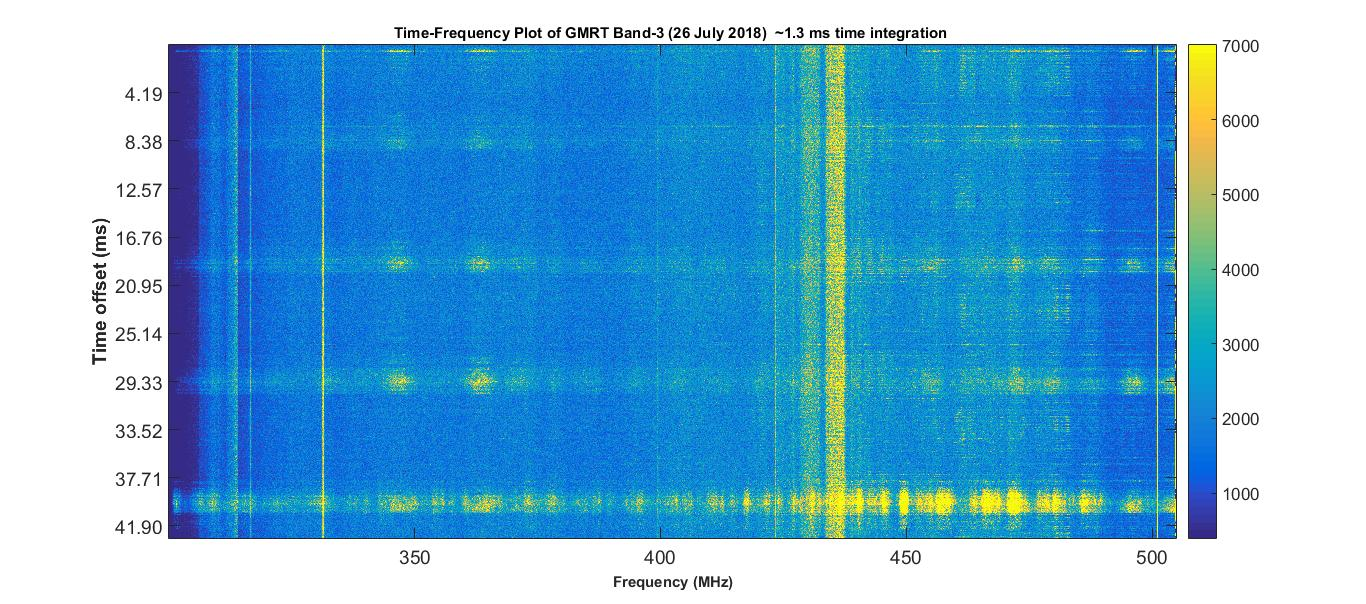
\includegraphics[scale=0.25]{Hardware Excision Techniques/figures/time_freq(1).jpg}
    \caption{Spectrogram of uGMRT \citep{gupta2017upgraded} antenna showing broadband (powerline RFI) and narrowband (communication transmitters) RFI in 250-500 MHz band. Broadband powerline RFI is seen to be repeating every 10ms (submultiple of 50Hz powerline frequency). Note that the astronomical signal is burried below the the noise floor and cannot be identified in this plot.}
    \label{fig:ugmrt-rfi}
\end{figure}




\subsection{Levels of RFI}
\label{subsection:hardware:introduction: levels}
A radio astronomy receiver chain begins with a feed that collects celestial radio waves, directing them to a low-noise amplifier (LNA). The LNA amplifies these weak signals with minimal added noise, ensuring data integrity. After amplification, the signal passes through a bandpass filter to isolate the frequency of interest, followed by downconversion, when applicable, to an intermediate frequency (IF) using a mixer and local oscillator. The IF or baseband signal is further amplified, filtered, and digitized by an analog-to-digital converter (ADC), though modern systems increasingly digitize directly at the RF frequency to minimize signal degradation.

Radio frequency interference (RFI) impacts the receiver chain at varying levels:
\begin{itemize}
\item \emph{Level 0}: Undetectable RFI does not impact observations, requiring long integration times to assess its threshold via modeling or experiments.
\item \emph{Level 1}: Detectable RFI adds unwanted contributions, requiring excision to preserve data integrity, but this can reduce sensitivity and hinder the detection of sparse astronomical signals or calibration accuracy.
\item \emph{Level 2}: Stronger RFI pushes the LNA into non-linear operation, generating harmonics and intermodulation products. Mitigation involves excising data and using attenuators, further degrading sensitivity.
\item \emph{Level 3}: Severe RFI causes ADC saturation, resulting in irrecoverable signal artifacts. Mitigation typically includes attenuators or high-dynamic-range ADCs but at the cost of sensitivity.
\item \emph{Level 4}: Extreme RFI physically damages receiver components, requiring the telescope to cease operation.
\end{itemize}
Spectrum management aims to ensure Level 0 RFI across primary radio astronomy frequency bands while recognizing that all levels of RFI may occur in non-allocated bands, depending on the telescope's environment. This balance reflects the ongoing challenges in protecting sensitive radio astronomy observations from both in-band and out-of-band emissions.


\subsection{Motivation for real-time RFI mitigation}
\label{subsection:hardware:introduction: motivations}

RFI mitigation in a radio observatory is carried out in different ways \citep{ford2014rfi}. Real-time RFI mitigation usually happens in the analog domain or at the highest time resolution, i.e. close to the Nyquist rate, which helps minimize the data corruption due to sparse RFI in downstream signal processing with minimal loss of astronomical data, thereby improving and enhancing the quality and accuracy of astronomical measurements. Figure~\ref{fig:real-time-rfi} illustrates the increase in data loss in a typical radio telescope receiver signal processing chain.
Other benefits from real-time RFI mitigation are as follows:

\begin{enumerate}
\item For time-domain impulsive RFI, the energy spreads across the observing band in the frequency domain, making it impossible to mitigate in the spectral or post-correlation domain.  See Figure~\ref{fig:rfi_example_radar} for an illustration with a radar system.

\item Correlated RFI is best treated in the pre-correlation domain to reduce its ill effects on the astronomical data.

\item RFI is mostly non-random; hence, its early removal helps follow the radiometer equation, which is crucial to achieving the desired sensitivity of the telescope.

\item It helps facilitate adjustments to the telescope signal processing chain in response to a dynamic RFI environment. This adaptability is crucial in maintaining the continuity of observations and ensuring that data collection is optimized even in transient or sporadic RFI.
\end{enumerate}

%\subsection{RFI classification}
%\label{subsection:hardware:introduction: classification}

\begin{figure}
    \centering
    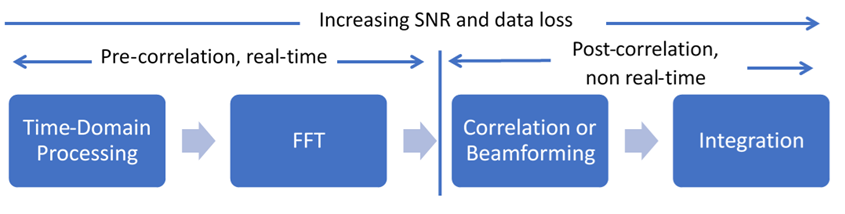
\includegraphics[scale=0.8]{Hardware Excision Techniques/figures/rt.jpg}
    \caption{SNR versus data loss in a typical telescope receiver system}
    \label{fig:real-time-rfi}
\end{figure}


\begin{figure}
    \centering
    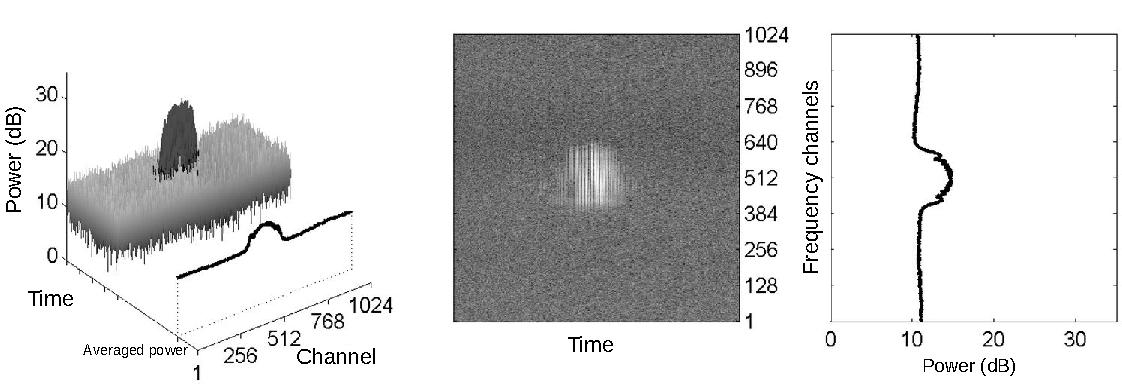
\includegraphics[height=.20\textheight]{figures/radar.pdf}
    \caption{One of the 5-s periodic bursts received from a radar system.  The burst is a group of many periodic short impulses, sparse in time, but broad.  }
    \label{fig:rfi_example_radar}
\end{figure}

%Additionally, real-time RFI mitigation contributes to the protection and longevity of sensitive receiver components by promptly handling high-power interfering signals and reducing the risk of thermal damage and long-term degradation of electronic components.
%While real-time detection and excision of RFI is beneficial in radio astronomy it comes with challenges. The main challenge is the cost and power consumption. Even though RFI has become a significant threat to radio astronomy for several decades, few signal chains of radio telescopes have been designed considering the real-time excision of RFI. Hence, the real-time RFI excision methods deployed in existing radio telescopes are implemented using the remaining resources after implementing the key signal processing modules and operated with limited power. Regarding quality, one of the main checks that needs to be made is the flagging duration and accuracy of flagging.  It should be ensured that the excision is optimal i.e. there is no over-excising of the data which can result in the loss of precious observational data or under-excising which leads to RFI remnants in the data.


%An example of a real-time RFI mitigation released and operational for the uGMRT including the possibility of extending it to contemporary and upcoming telescopes is provided in \citep{buch2023real}.


%\subsection{Advantages of Real-Time RFI Excision}
%\label{subsection:hardware:introduction:advantages}

%Advantages of Real-Time RFI Excision
%Improved Data Quality: By removing RFI in real-time, astronomers can obtain cleaner data, which can lead to more accurate and reliable scientific results.
%Reduced Storage Requirements: Removing RFI before data is stored can significantly reduce the amount of storage space required, as only the cleaned data needs to be preserved.
%Real-Time Monitoring: Real-time excission allows astronomers to monitor the data quality as it is being collected, enabling them to identify and address potential issues promptly.
%Efficient Data Analysis: Clean data is easier and more efficient to analyze, as it is less likely to be contaminated by artifacts or noise.
%Reduced Computational Burden: By removing RFI before data is analyzed, astronomers can reduce the computational resources required for subsequent processing.

%\%subsection{Challenges of Real-Time RFI Excision}
%\label{subsection:hardware:introduction:challenges}

%Disadvantages of Real-Time RFI Excision
%Algorithm Complexity: Developing accurate and efficient algorithms for real-time RFI excission can be challenging, especially for complex RFI patterns.
%Computational Overhead: Real-time excission can introduce computational overhead, which may limit the data throughput of the telescope.
%Risk of False Positives and Negatives: There is a risk of mistakenly removing genuine astronomical signals or leaving RFI in the data, which can impact the scientific interpretation.
%Dependency on Algorithm Performance: The effectiveness of real-time RFI excission depends heavily on the performance of the algorithms used, which can be affected by factors like the type and severity of RFI.
%Potential for Data Loss: In some cases, aggressive RFI excission can lead to the loss of genuine astronomical signals, particularly if the RFI is difficult to distinguish from the signal.


%\subsubsection{Thushara}
%Real-time RFI excision enables radio astronomers to salvage observations taken in a contaminated segment of the observation band, either when the RFI source is not transmitting or when the RFI strength is attenuated to a level below the ITU recommended threshold\citep{ITU_protection_2003}. For example, consider the interference caused by strong radio pulses emitted by the Distance Measuring Equipment (DME) of an aircraft \citep{wiki_dme_2024}, which are being picked up by the antennas of radio telescopes. The DME pulses transmit in bands within 960-1215 MHz at a power level of 1 kW. Each DME pulse is 3.5 µs wide and repeats every 12 µs for a second or so in a single burst. Normally, the DME pulses are detected by the sidelobes of the antennas of a radio telescope. These pulses can be fairly easy to detect at the front of the signal chain of the radio telescope, which is operating at a wider bandwidth. Once detected, the contaminated data can be flagged in real-time to prevent further contamination of the accumulation. Also, RFI detection carried out along the various stages of the signal chain of a radio telescope allows radio astronomers to maintain the linearity of the signal chain with proper scaling while achieving the maximum possible dynamic range for a given set of computational resources.

%While real-time detection and excision of RFI is beneficial in radio astronomy it comes with challenges. The main challenge is the cost and power consumption. Even though RFI has become a significant threat to radio astronomy for several decades or so few signal chains of radio telescopes have designed considering the real-time excision of RFI. Hence, the real-time RFI excision methods deployed in existing radio telescopes are implemented using the remaining resources after implementing the key signal processing modules and operated with limited power. In terms of quality, one of the main drawbacks of real-time RFI excision is the uncertainty of the flagging duration.  This leads to either over-excising the data resulting in the loss of precious observations or under-excising which leads to RFI remnants causing artifacts in the observations. 

%\subsubsection{Kaushal - Motivation for Real-time RFI Mitigation}

%Real-time RFI mitigation usually happens at the highest time resolution (Nyquist rate) which helps prevent data corruption in downstream signal processing with minimal loss of astronomical data. Other benefits from real-time RFI mitigation are as follows:

%1. For time-domain impulsive RFI, the energy 
%spreads across the observing band upon Fourier
%transformation, making it difficult to detect and
%mitigate in the post-processing operation.

%2. Mitigation in the pre-correlation domain helps
%reduce the ill effects of correlated RFI.

%3. RFI is mostly non-random and hence its early removal helps in following the radiometer equation which is crucial to achieve the desired sensitivity of the telescope.

%\subsubsection{Greg}
%Real-time RFI mitigation is a critical capability of modern radio telescopes that facilitates adjustments to the telescope signal processing chain in response to a dynamic RFI environment. This adaptability is crucial in maintaining the continuity of observations and ensuring that data collection is optimized despite the presence of transient or sporadic RFI. It also enhances the quality and accuracy of the collected astronomical information by identifying, attenuating, or excising corrupted data at the highest data rates before any data compression, and preventing the saturation of the vulnerable receiver components (e.g. LNA or ADC).

%Mitigating RFI in real-time also helps minimizing the downstream computational load and storage requirements by processing the RFI contribution at the point of data acquisition rather than further down the signal chain. This strategy alleviates the need for storing intermediate data products, which can be unbearbel with the increase of telescope bandwidths and array sizes.

%Additionally, real-time RFI mitigation contributes to the protection and longevity of sensitive receiver components by promptly handling high-power interfering signals and reducing the risk of thermal damage and long-term degradation of electronic components.



\section{Catalog of real-time mitigation techniques}
\label{section:hardware:catalog}

\subsection{Existing real-time implementations}
\label{subsection:hardware:catalog:existing}
\subsubsection{Preventive : Avoidance}
Most radio telescopes operate in an automated fashion, following a scheduler. The locations of known fixed sources of RFI, such as terrestrial emitters and geostationary satellites, are well-established. These fixed sources can be factored into the telescope's schedule, allowing for optimized observation strategies that minimize the impact of RFI on collected data. This is achieved by aligning the telescope's sequence of sky pointings with a model of its directivity pattern, avoiding these known interference sources.

In a more dynamic approach, the telescope can also avoid known moving sources of RFI, such as medium Earth orbit (MEO) satellites and aircraft. Satellite position data is publicly available, and aircraft locations can be tracked using ADS-B transmissions. However, avoiding low Earth orbit (LEO) satellites poses a greater challenge due to their high angular speeds and sheer numbers.

Dynamic interference avoidance strategies are being proposed for next-generation telescopes like FAST, ngVLA, and DSA-2000. ASKAP is also developing an RFI avoidance scheme to address atmospheric ducting events, which can channel RFI over large distances

\subsubsection{Analog: Adaptive analog attenuators LWA (Greg)}

\subsubsection{Superconducting filters (YEBES)}
We only have hardware-based techniques in the form of high-temperature superconducting (HTS) filters in front of the low-noise amplifiers.
Some filters show resonances (spurious responses) at other frequencies in the band of the receiver.
the filters can’t be automatized as they are always present.

F. Huang et al., “Superconducting spiral bandpass filter designed by a pseudo‐Fourier technique,” IET Microwaves, Antennas \& Propagation, vol. 12, no. 8, pp. 1293–1301, Apr. 2018, doi: https://doi.org/10.1049/iet-map.2017.0940.
Ph.D. thesis by Pablo Garcia-Carreno: “Optimización de receptores criogénicos mediante filtros superconductores para supresión de interferencias y sistema de medida de la fase de la señal de referencia”. https://ebuah.uah.es/dspace/handle/10017/59826?locale-attribute=es
New filters to be published soon (papers in progress).


\subsubsection{Analog: GMRT (Kaushal)}

Strong narrowband RFI from various sources that affect the upgraded GMRT receiver’s dynamic range and linearity are mitigated using band reject/notch filters. These are incorporated in the front end of the receiver system to ensure that the system operates in the linear region by rejecting strong and persistent RFI from strong short-range transmissions, mobile communication, and broadcast television \cite{sureshkumar2016rfi}. Efforts to use the latest techniques to have the filter before the LNA are being developed to avoid saturation due to strong interfering signals.

\subsubsection{Analog: switchable notch filters Green Bank}
\subsubsection{Digital: switch ADC fromm 3 to 12 bits at Green Bank}

\subsubsection{Digital: Excision in time}

\begin{itemize}
\item Real-time RFI Excision at GMRT (Kaushal)

The upgraded GMRT (uGMRT) \cite{gupta2017upgraded} operates from 120 to 1450 MHz and has near-seamless coverage in this band. It is an array of 30, 45m diameter parabolic dishes and a sensitive receiver which operates in the interferometry and beamformer modes. The array is located 80 km north of Pune in India. The increase in the population around the array in the last 30 years along with the proliferation of communication devices, satellites, and mobile phones, has caused an increase in the RFI. The uGMRT signal processing backend has a real-time RFI excision system for mitigating RFI and achieving sensitivity levels close to the theoretical limits. \\

\begin{figure}
    \centering
    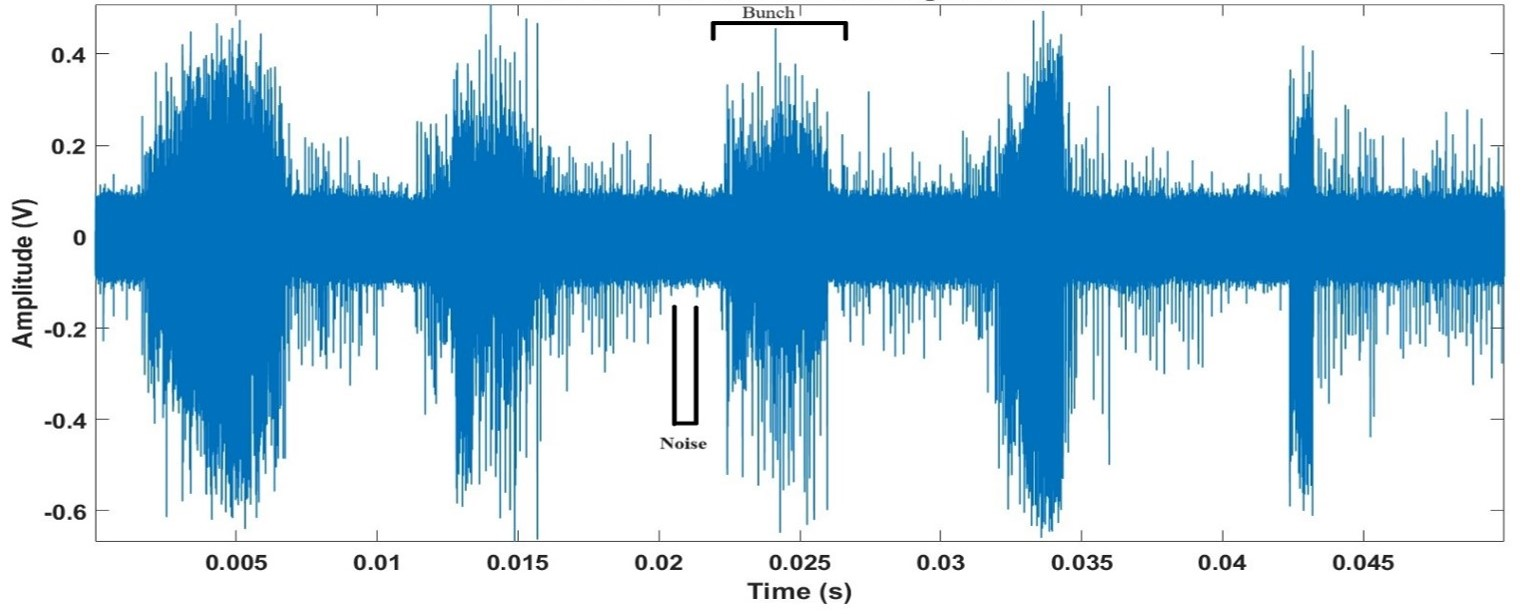
\includegraphics[scale=0.7]{Hardware Excision Techniques/figures/Band4_timeseries_ed.jpg}
    \caption{A 50ms time-series of single antenna Band-4 (550-850 MHz) data. Powerline RFI can be seen to occur in bunches repeating every 10ms. The data is acquired at the input of the signal processing system with a time resolution of 5ns.}
    \label{fig:ugmrt-b4-ts}
\end{figure}

One of the main causes of RFI at frequencies less than 1 GHz is sparking and corona discharge on the high-tension lines and transformer installations around the array. This type of RFI is impulsive in the time domain (Ref. Figure~\ref{fig:ugmrt-b4-ts}) resulting in a broadband increase in the power in the spectral domain. Since this type of RFI cannot be mitigated by frequency selective filters in the receiver system, a real-time statistical RFI excision system was developed which operates on digitized time-series from each antenna and polarization. This system is designed to excise strong impulses in the received signal. \\

The real-time system currently implemented on FPGA \cite{buch2019real} uses a median-based robust estimation and threshold detection scheme. Each incoming sample (at Nyquist rate) is compared with a robust threshold and samples detected as RFI are replaced with a constant value, threshold or digital noise sample. After rigorous testing on various astronomical data products, the RFI system is released for observations and is currently extensively used for observations in the lower frequency bands of uGMRT (< 1GHz). An example of imaging through this system wherein half the antennas used the original signal whereas the other half used the filtered copy \cite{buch2022performance} is shown in Figure~\ref{fig:ugmrt-b4-image}. \\

\begin{figure}
    %\centering
    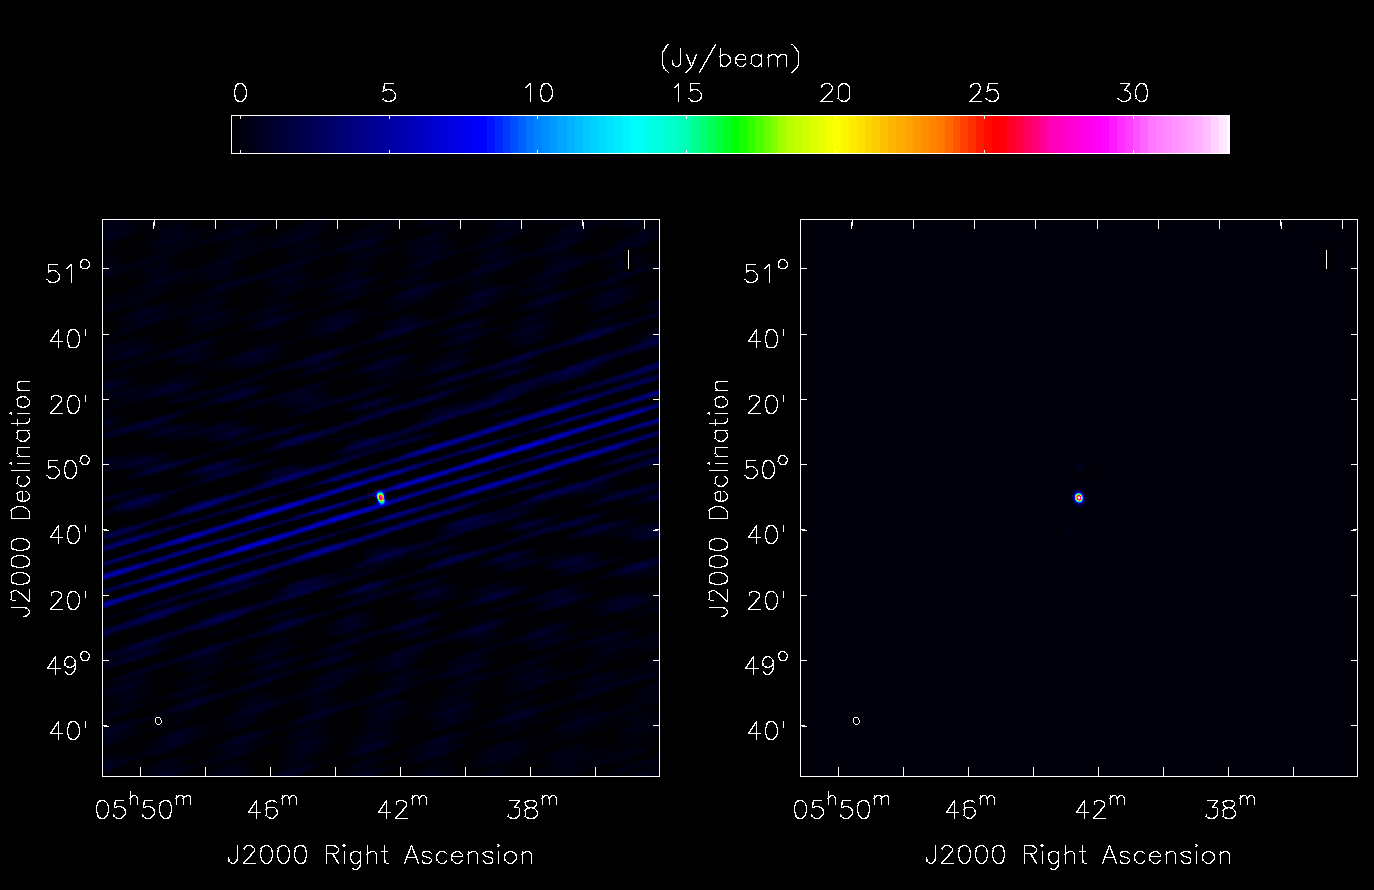
\includegraphics[scale=0.4]{Hardware Excision Techniques/figures/band4_point_source_rfi_filtering.png}
    \caption{uGMRT image, 9 antenna, point source 3C48 observed in band-4 (550-850 MHz). The image is built using baselines $<$0.5km and tested simultaneously to see the effects of real-time RFI filtering. The image corrupted by broadband RFI (left) is improved by a factor of 3 in the filtered version (right). Image courtesy: Ruta Kale, NCRA, India.
}
    \label{fig:ugmrt-b4-image}
\end{figure}

A possibility of refinements to the technique including mitigating low-level RFI, using learning-based approaches, and implementing similar techniques in real-time for mitigating narrowband RFI \cite{buch2016real} is being looked at. The technique is also being proposed \cite{buch2023real}for upcoming telescope like the SKA.\\


\item post-PFB (LWA+DSA-2000 - Greg)
\end{itemize}

\subsubsection{Digital: Excision in spectral}
\begin{itemize}
\item AOFlagger-type Westerbork (Greg)

 RFIm \cite{sclocco2019real} is an open-source, high-performance library designed to mitigate RFI in real time. RFIm is optimized to run on many-core accelerators such as GPUs and provides methods that are robust yet computationally efficient. The library features two main algorithms: Time-Domain Sigma Cut (TDSC) and Frequency-Domain Sigma Cut (FDSC). These two algorithms detect and replace RFI-contaminated data with statistical averages to reduce false positives without significant impact on processing time. This approach allows systems like the Apertif Radio Transient System (ARTS) to maintain high data throughput while effectively identifying real astronomical signals amidst increasing anthropogenic and satellite-generated interference.
 
\item Higher-order statistics at EOVSA (Greg)

The Spectral Kurtosis (SK) technique is a statistical method used for real-time detection of non-Gaussian signals, such as radio frequency interference (RFI), within Gaussian noise in radio astronomy data. The SK estimator distinguishes signals by comparing power and power-squared values of spectral data to detect deviations from Gaussian behaviour. The Expanded Owens Valley Solar Array (EOVSA) implements this SK technique in its correlator, using an FPGA-based system to perform real-time SK calculations directly within the Fourier transform engine \cite{}. This design allows the system to flag and exclude contaminated data dynamically, enhancing the quality of observations by effectively identifying and mitigating RFI while preserving genuine astronomical signals.

\item MeFisTo: Frequency and Time Median filter on Nançay Decameter Array (Cedric)

Between 5 and 88 MHz, the lowest part of the frequency band accessible to ground-based telescopes, the sky is crowded with audio and timing broadcast users, allocated to frequency channels much closer than the frequency resolution required to meet the scientific needs of solar and Jovian observations. This band is also affected by wideband RFI generated by electric fences, spark ignition systems from internal combustion engines, and power lines.

Time and frequency analysis of this band must be performed with temporal and spectral resolutions far exceeding the requirements for scientific observations. This results in data streams and data sets much larger than necessary for scientific purposes.

Since 2013, a receiver \cite{lecacheux2013, 2017pre8.conf..455L} based on 80-MSps ADCs and a Stratix IV FPGA has implemented a real-time streaming Blackman-Harris-windowed 64k-FFT, followed by classical (averaged) time-frequency analysis using a Welch-averaged periodogram. Simultaneously, the same periodogram is computed with a median filter (kernel size=64) applied first on the frequency axis, then on the time axis (kernel size=128), to mitigate narrowband and wideband RFI in observations. The frequency resolution for RFI mitigation is as low as 1.2 kHz, but it is raised to 78 kHz for scientific purposes. The time resolution for RFI mitigation is 0.8 ms but is increased to 104 ms to provide a sustainable data rate for 24/7 monitoring of the Sun and Jupiter.

\begin{figure}
    \centering
    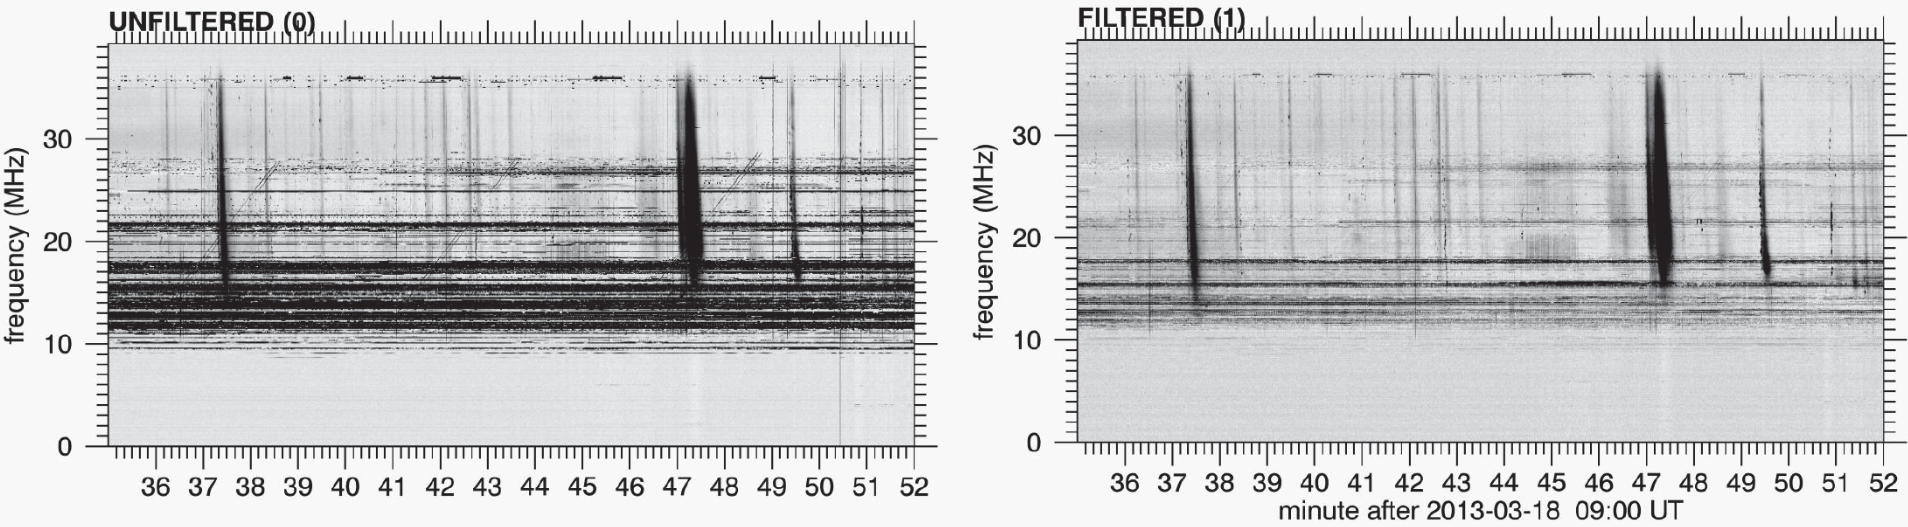
\includegraphics[width=\textwidth]{figures/MeFisTo.png}
    \caption{Solar activity observed without (left) and with (right) RFI median TF-filtering.  Wideband RFI and ionospheric sounders are eliminated, and shortwave broadcasts are significantly attenuated. \cite{lecacheux2013}}
    \label{fig:rfi_MeFisTo}
\end{figure}


\item RFI mitigation implementations on RDH at Nançay (Cedric)

In the early 20th century, a configurable digital receiver was deployed at the Nançay Observatory. The receiver's ADC+FPGA+DSP system was shared by the 100-meter Decimeter Wavelength Telescope (NRT) and the Decameter Wavelength Analog Phased-Array (NDA). The main purpose of this receiver was to develop operational techniques for RFI mitigation. This hardware is now largely obsolete and was decommissioned years ago. However, the techniques remain and may be reused in future deployments.

The core work in designing these operational RFI mitigation techniques relies on a detailed study of the statistical behaviour of operators that can be easily implemented in real-time digital logic to create robust mean power estimators \cite{dumezviou:tel-00319939}. This toolbox can then be used to develop custom implementations that address the challenges encountered in the design of digital receivers for radio astronomy.  Next, two implementations are presented:

\begin{itemize}
\item HI red-shifted radio galaxies have the rest frequency of the hyperfine transition at 1420 MHz shifted into frequency bands allocated to L-band radar systems used for civil and military aircraft detection and ranging. Every 5 or 10 MHz, a radar system emits several kilowatts of power for one microsecond, with a pulse rate period of one millisecond. Theoretically, the sky is clear during the remaining 999 microseconds and available for astronomical observations. Detecting strong radar pulses with SNRs tens of dB above system noise is straightforward. The challenge lies in detecting weak pulses with negative-dB SNRs while maintaining an acceptable false alarm rate.

This was successfully implemented in the very limited resources of Virtex II FPGAs using the previously mentioned toolbox, allowing the excision of data blocks contaminated by both weak and strong radar pulses before they are passed to the spectral analysis block. As a result, HI surveys can now be conducted without artifacts originating from radar systems.


\item Red-shifted OH mega-masers may have their 1665 and 1667 MHz lines fall into the band the Iridium satellite constellation uses. This system manages access to the radio spectrum through a TFDMA scheme. During the test campaign, only a few percent of the millisecond-scale instantaneous spectrum was occupied, but after a few seconds of integration, the entire band became corrupted.

Spectral analysis was configured to generate data with time and frequency resolutions (3.4 kHz and 2.34 ms) tailored to the TFDMA characteristics. A MAD-estimated power criterion was then applied to discriminate between corrupted and pristine data slots, removing RFI from the dataset before integration.

\begin{figure}
    \centering
    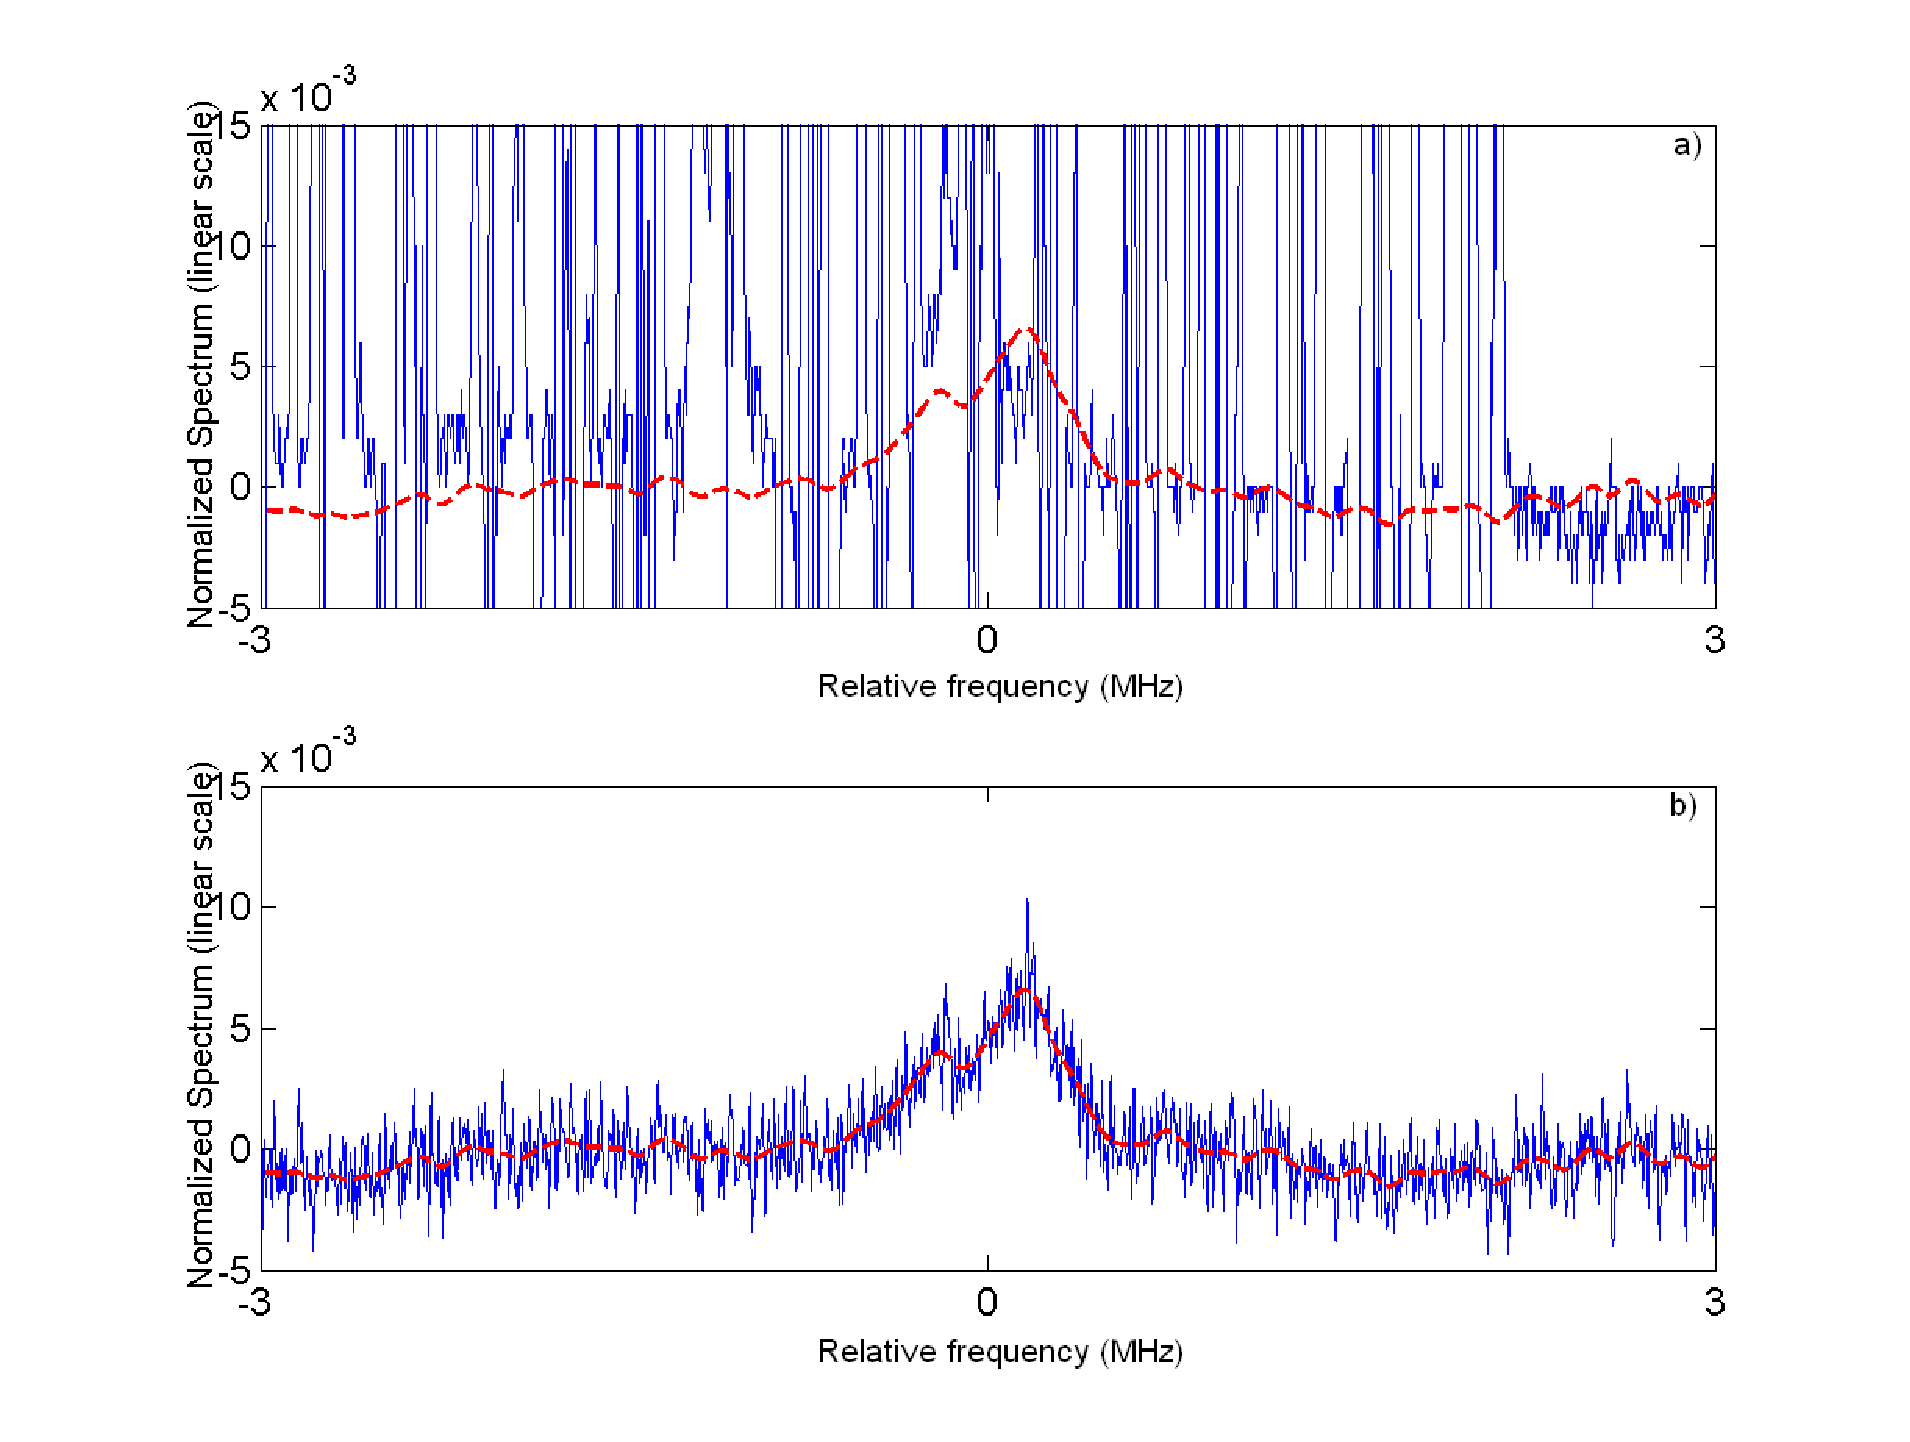
\includegraphics[height=.28\textheight]{figures/IIIZw35_20040108.eps}
    \caption{Re-observation of III Zw 35 on January 8, 2004, in real-time after 14 minutes of integration with the NRT: (a) Without "blanking." The vertical axis is adjusted to make the expected source profile visible. (b) With "blanking" (3.5\% of data eliminated). The source is visible again.}
    \label{fig:rfi_Iridium_blanked}
\end{figure}

This was implemented on TMS 6203 TI DSP chips to process the frequency band in real time.
\end{itemize}


(Thushara)
\item CHIME: The Canadian Hydrogen Intensity Mapping Experiment \href{https://chime-experiment.ca/en}{(CHIME)} is a radio telescope primarily designed to study the distribution of neutral hydrogen gas in the Universe. Serendipitously, it turned out to be an excellent instrument for detecting fast radio bursts (FRBs), the mysterious millisecond-long radio flashes of unknown origin. When processed with the CHIME FRB pipeline, strong impulsive RFI may lead to false positives and therefore needs to be mitigated \cite{chime_frb_rfi_2023}. Several real-time iterative processes have been applied iteratively to weed out the statistical outliers from the channelized intensity data that are effectively high-pass filtered.

The RFI mitigation process before the dedispersion transform in L1-pipeline for CHIME/ FRB search is explained in \cite{chime_frb_rfi_2023}. The channelized intensity data of each beam are processed by 'subpipeline' containing alternate \textit{Clipping transforms} and \textit{Detrending transforms chains}. There are two different clipping transforms: intensity and standard deviation clipping transforms, to mask the statistical outliers in the intensity data. Every clipping iteration helps
improve the RFI mask by recognizing more statistical outliers and hence reshaping the masked intensity PDF to a robust $\chi^2$ distribution in real time. The large-scale variations from RFI, forward gains, and digital beamforming are seen in the CHIME/FRB intensity time series as functions of the time, frequency, and sky location. Due to the distorted intensity PDF, the clipping and dedispersion transforms fail. The proposed detrending transforms provide a computationally less-intensive way of high-pass filtering in the harmonic space of intensity.



\item MeerKAT: correlator dumps outlier excision at high time res (ingest step, see Sihlangu and Ludwig)
The ingest stage directly after the MeerKAT correlator has a fast and simple “1-D” mean absolute deviation (MAD) filter (“ingest\_rfi”) which identifies the background by running along the frequency axis and thresholds each dump and correlation product independently. It runs on a GPU and is conservatively tuned to identify obvious spikes in amplitude, flagging roughly 4\% of the data in the L band. This applies to all imaging modes but not pulsar mode, which has its own RFI mitigation scheme.
Initially, the ingest stage also excised data that was flagged by the “ingest\_rfi” filter before it averaged 0.5-second raw correlator dumps to the final 8-second dumps. Scientists did not like this idea (and RFI researchers even more so!), so it was canned.

The majority keep the more conservative “ingest\_rfi” flags but not the more aggressive “cal\_rfi” flags. Observers that take our pipeline images will have all flags applied.

The main codebase for our flagger is https://github.com/ska-sa/katsdpsigproc. The tricolour MeerKAT flagger is a similar standalone flagging package. See https://arxiv.org/abs/2206.09179.


\item MeerKAT: calibration step VarThreshold  (see Sihlangu and Ludwig)
The calibration pipeline which follows after ingest has a more advanced “2-D” flagger (“cal\_rfi”). It is a tweaked AOFlagger written from scratch in Numba. It identifies the background by running along both the time and frequency axes. It performs two passes, first finding a smooth background on previously unflagged parts and then sum-thresholding. It only flags HV and VH (cross-hand) data and extends the results to HH and VV. It flags the calibrator before solving for gains, and it flags the target after applying gain corrections to it, which allows more stringent flagger parameters. It typically flags about 20\% of the data in the L band. This applies to all imaging modes but not pulsar mode, which has its own RFI mitigation scheme.


\end{itemize}

\subsection{Prospective real-time implementations}
\label{subsection:hardware:catalog:prospective}

\subsubsection{Preventive: Dynamic scheduler (Greg)}
\subsubsection{Preventive: satellite avoidance at Green Bank}
Satellite boresight avoidance is a technique to prevent satellites from directly illuminating a telescope's primary observation direction. In experiments conducted by the Green Bank Telescope (GBT) with Starlink satellites, this technique was tested \cite{nhan2024spectrumcoexistencedemonstrationeffectiveness} by adjusting the satellite constellation's configuration based on real-time telescope pointing data and predicted satellite trajectories. This approach minimizes interference by dynamically coordinating telescope operations with satellite activities, such as emission control and beam steering. The process is facilitated by the Operational Data Sharing (ODS) system, an autonomous platform developed by the National Radio Astronomy Observatory (NRAO). ODS provides satellite operators with real-time updates on telescope positions and observing frequencies, allowing them to adjust satellite operations accordingly. With frequent updates, potentially every minute, ODS ensures effective coordination, especially during close satellite passes near the telescope’s boresight

%\subsubsection{Analog: Notch filters for uGMRT (Kaushal)}
\subsubsection{Analog : Tunable notch filter DSA-2000 (Greg)}

The tunable notch filters are designed to mitigate RFI in the analog front end of the DSA-2000 receivers. The Quad-Stub Resonator Filter uses four high-Q “series LC” stubs, each controlled by voltage-tuned varactors, allowing independent frequency tuning for precise RFI mitigation. The filter achieves deep notch attenuation, adjustable within a range of 550 MHz to 1050 MHz, with peak attenuation up to 62.5 dB. It features a chassis design with RFI-tight seals and SMA connectors to prevent interference coupling. The filter's response is fine-tuned through individual varactor bias adjustments, enabling adaptable and effective RFI suppression across a broad frequency range.

\subsubsection{Analog: Reconfigurable Intelligent Surface (Greg)}

Reconfigurable Intelligent Surfaces (RIS) can mitigate RFI at the telescope receiver by dynamically shaping the electromagnetic wavefronts to create a destructive interference zone around the receiver \cite{zou2022scisrs,wei2024ris,wei2023multistage}. The RIS array, composed of multiple controllable elements, adjusts the phase and amplitude of reflected signals to precisely counteract incoming RFI. By steering reflected signals from the RIS in such a way that they are out of phase with the incident RFI, the RIS effectively cancels the RFI energy before it reaches the telescope’s receiver. This approach allows for the creation of an electromagnetic quiet zone, enabling the telescope to perform sensitive astronomical observations without interference from external RFI sources, such as aircraft and satellites, without altering the telescope’s primary astronomical signals.

\subsubsection{Digital: SK EDD Effelserg}
\subsubsection{Digital: cyclic spectroscopy Green Bank}

\subsubsection{Digital: Excision in time parametric subtraction Ellingson (Greg)}

The time-domain coherent cancellation (CTC) technique is a method used to mitigate RFI by subtracting an interference estimate from the received signal in real-time \cite{ellingson2022coherent}. CTC operates by generating a reference signal that represents the interfering source, which can be acquired externally (e.g., through a separate antenna) or synthesized internally using prior knowledge of the interference. The reference signal is used to create an interference estimate that is coherently subtracted from the received signal, ideally leaving only the astronomical signal of interest with minimal added noise or distortion. The approach allows telescopes to "look through" interference, preserving affected data that would otherwise be discarded by traditional methods, though it requires precise estimation and synchronization to avoid errors that could compromise the scientific data.

\subsubsection{Digital: Threshold-based pre-correlation RFI detection technique to be used in SKA.Mid (Thushara)}
\label{subsection:hardware:catalog:ska-mid}

The Correlator Beamformer for the Mid-frequency telescope for the \href{https://www.skao.int/en}{Square Kilometre Array} (SKA-Mid.CBF) uses a 'power threshold-based' RFI detection scheme \cite{ska_mid_cbf_rfi_2019}. The main objective is to preserve the linearity of the signal chain while achieving the desired dynamic range to maintain the sensitivity. The architecture of the proposed RFI detector/flagger module is shown in Figure~\ref{fig:rfi_df_ska_mid_cbf}. As shown there, two-time scales are involved:
\begin{enumerate}
    \item Long-term ($>$1 sec, considering on/off state of the noise diode) for establishing an average power level, and
    \item Short-term to detect and flag bursting RFI to prevent downstream spectral splatter.
\end{enumerate}

The number of samples used for the short-term power calculation is programmable. If the short-term power calculation is greater than a programmable threshold, set by the Telescope-Manage or internally determined if “auto-set”, then a flag is set and carried with the data stream to the downstream processing module, and downstream operations (i.e. any that affect output data products or intermediate calculations needed such as gains/levels settings) are inhibited for the number of samples that it takes the flag to propagate through all downstream processing modules. As per the flagging policy, both polarization components are flagged if one is flagged. The dwell time of the flag is also programmable to balance the data loss with the risk of contamination. Note that the flagged data is not used in evaluating the long-term power calculation to have an estimate of the signal level of the non-RFI-contaminated signal. The long-term power is accumulated in two separate bins, one for noise diode on, and one for noise diode off.

\begin{figure}
    \centering
    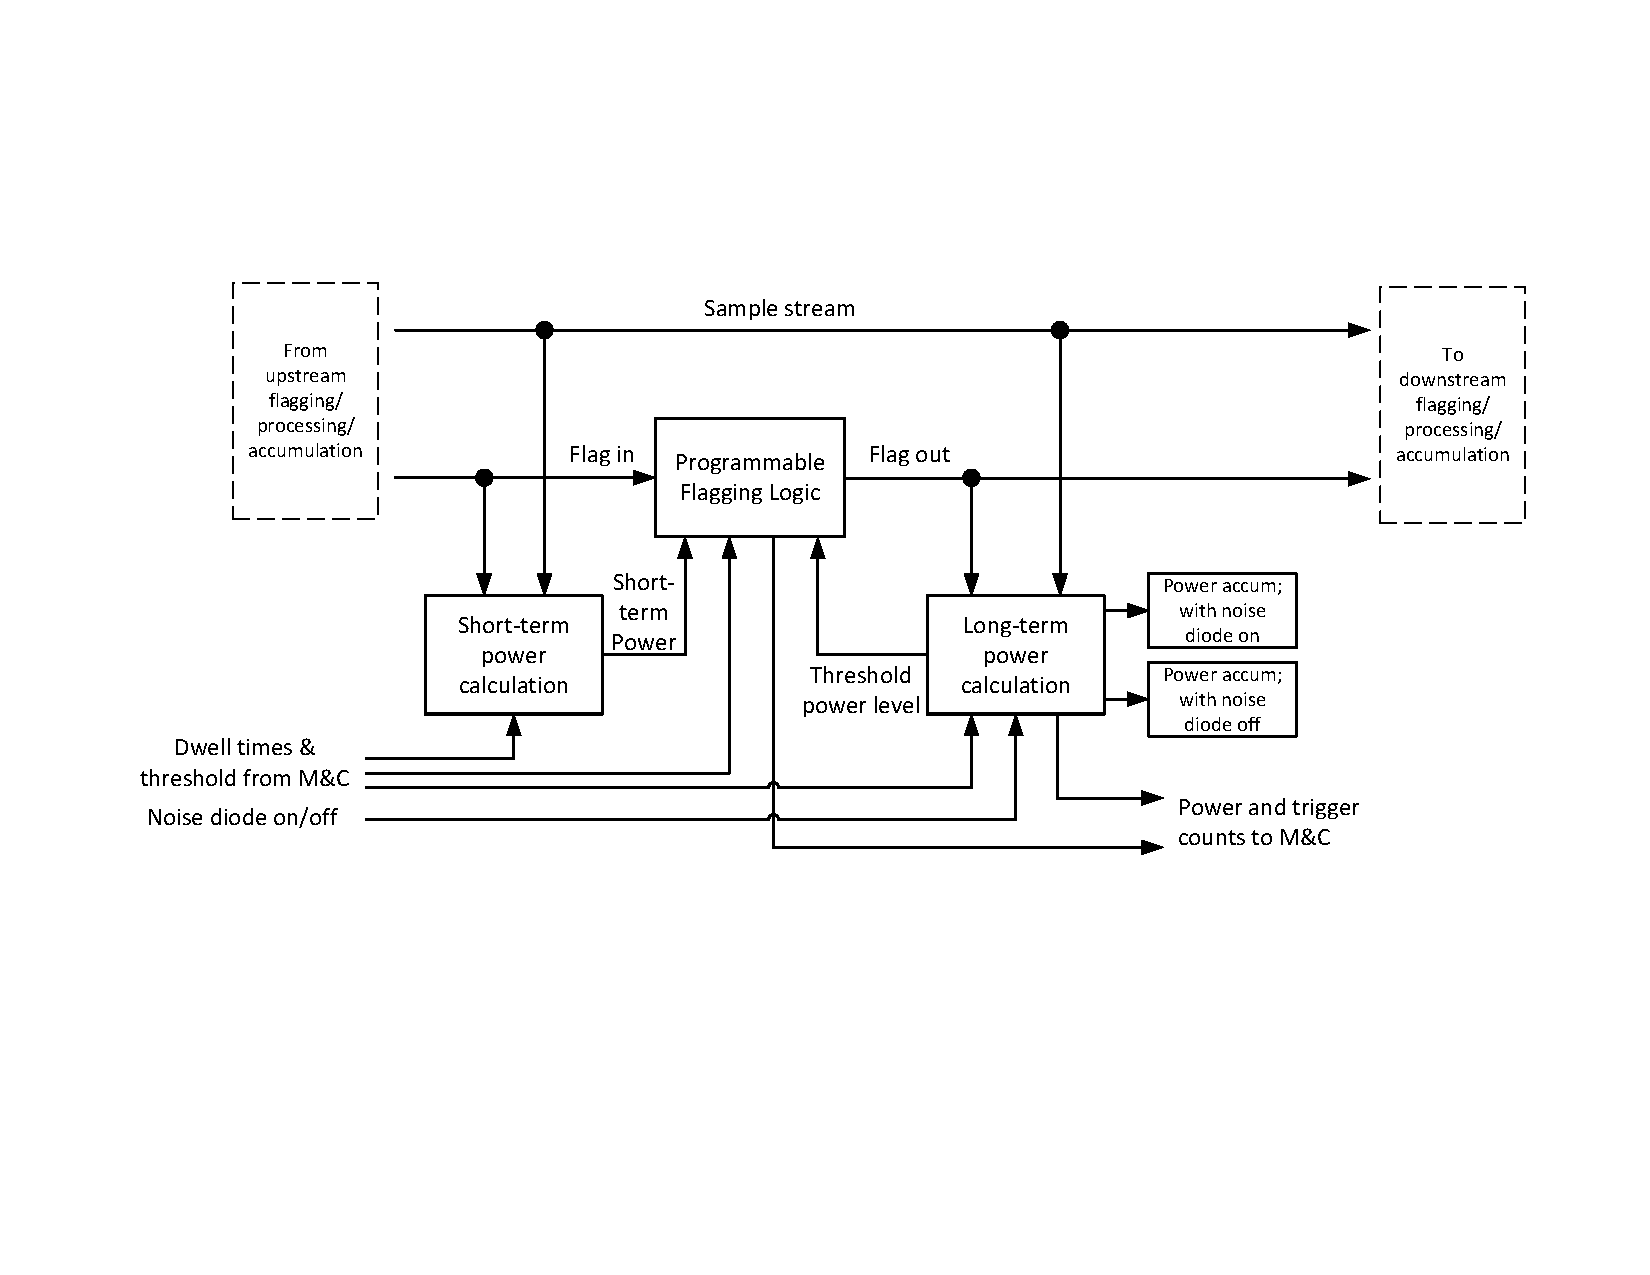
\includegraphics[height=.28\textheight]{figures/RFI_DF_SKA_Mid_CBF.pdf}
    \caption{The proposed RFI threshold detector/flagger (from \cite{ska_mid_cbf_rfi_2019}).}
    \label{fig:rfi_df_ska_mid_cbf}
\end{figure}


\subsubsection{Digital: excision in UV domain (Greg)}

GRIDflag \cite{10464448} is a UV-plane-based RFI flagging algorithm designed to enhance the sensitivity and imaging fidelity of radio interferometric observations in the presence of strong and persistent RFI. Unlike traditional methods that flag RFI in the time-channel plane of baselines, GRIDflag operates directly in the UV plane, where multiple baselines sample similar spatial Fourier components redundantly across a regular grid. By statistically comparing UV samples within each grid pixel, GRIDflag identifies and flags RFI-affected points, preserving UV coverage and sensitivity to spatial scales. This approach is particularly effective in mitigating systematic noise introduced by faint RFI, which can otherwise degrade image sensitivity and accuracy. GRIDflag's design allows it to be computationally efficient and adaptable to modern technologies like GPUs, making it well-suited for current and next-generation radio telescopes.

\subsubsection{Digital: Spatial filtering (Greg, Kaushal)}
\begin{itemize}
\item Classic spatial filtering

The core idea is to leverage the spatial diversity of RFI and astronomical signals, along with the unique spatial signatures of interfering sources, to separate and suppress RFI \cite{hellbourg2014radio,hellbourg2016spatial,hellbourg2014rfi}. By estimating the RFI subspace using techniques like Singular Value Decomposition (SVD) and exploiting cyclostationary properties of RFI signals, spatial filters are designed to project received signals onto subspaces orthogonal to the RFI, effectively nulling interference. These filters can be applied either before or after correlation stages in the data processing chain. The technique is particularly valuable for modern radio telescopes, such as LOFAR and EMBRACE, where dense antenna arrays provide numerous redundant measurements, enhancing the precision of RFI mitigation without significantly impacting the desired astronomical signal. This approach helps maintain high fidelity and sensitivity in observations despite increasing RFI challenges from human-made sources.

\item Reference-antenna

A reference antenna can be used to mitigate RFI in real-time by providing an accurate estimation of the RFI spatial signature, which can then be used for spatial filtering in radio astronomy. The reference antenna is positioned to specifically capture the RFI without significantly receiving the astronomical signals. This RFI reference signal is correlated with the signals received by the main telescope array, allowing the RFI's spatial signature to be extracted and identified. This information is then used to project out the RFI from the main array's data using spatial filtering techniques, such as subspace projection.

By continuously updating the RFI spatial signature using subspace tracking algorithms, like the Power Method or Rayleigh Quotient Iteration, the system can adapt to changes in the RFI environment in real-time, effectively cancelling out the interference without impacting the astronomical signals. This approach is particularly effective for managing multiple RFI sources and dynamically changing interference patterns, enabling high-fidelity observations even in heavily contaminated radio bands\cite{hellbourg2014reference,sardarabadi2015spatial}.

\end{itemize}
\subsubsection{Digital AI/ML} (Greg, Kaushal)
\begin{itemize}
\item Collaborative Signal Subtraction (Greg)

The collaborative approach to RFI mitigation works by establishing a bidirectional communication between radio telescopes and interfering sources, such as cellular networks, to actively share RFI information and cancel interference in real-time. The interfering sources decompose their signals into a compact representation using techniques like the Karhunen–Loève Transform (KLT), which captures the signal's statistical properties independent of time and frequency. This RFI information, including eigenfunctions representing the interference, is periodically shared with the telescope through a low-overhead communication channel.

At the telescope, the received composite signal, which includes both astronomical signals and RFI, is similarly decomposed. The shared RFI characteristics are then used to cancel the interference from the telescope’s data through orthogonal projections in the eigenspace, thereby revealing clean astronomical signals. This approach significantly reduces communication and computational overhead by prioritizing the sharing of high-impact RFI data and selectively updating the interference model based on its influence on the telescope, thus maintaining high accuracy in signal recovery while managing multiple RFI sources effectively \cite{chakraborty2023collaboration,chakraborty2024low}.

\item Pattern recognition (Greg)

Automated pattern recognition to identify RFI in real-time radio astronomy data \cite{Winkel_2007} uses edge detection and window fitting to isolate high-intensity regions in the time-frequency domain, likely corresponding to RFI. Statistical analysis then helps differentiate RFI from genuine astronomical signals by comparing intensity patterns and variations. Iterative baseline fitting further refines the detection to ensure that RFI is accurately identified without impacting the integrity of the astronomical data. This method can be implemented in real-time systems, enabling dynamic flagging and mitigation of RFI, which is crucial for maintaining data quality in environments prone to interference, such as those near populated areas or satellite systems.

\item External flag generation (RFI monitor?) (Greg)

An RFI detector can provide real-time flags for radio telescopes by using machine learning techniques to automatically identify and classify interference in the radio frequency spectrum. The system described here \cite{9111666} employs a deep neural network (DNN) that processes time-frequency data, detecting and drawing bounding boxes around RFI events. This approach allows the detector to continuously monitor the RF environment and flag novel or anomalous RFI events in real time. The detected RFI events are flagged based on their spatial, spectral, and temporal characteristics, allowing the telescope to dynamically adjust its data processing pipeline to exclude or compensate for contaminated signals.

By integrating with the telescope’s data stream, the system can provide immediate notifications about RFI, enabling telescopes to respond promptly to interference without manual intervention. This real-time detection capability is particularly useful for maintaining the quality of astronomical observations by preventing the degradation of data due to unwanted interference.

\item Real-time RFI Prediction for Satellite RFI at GMRT

For spatially confined sources of interference that affect the GMRT for a fraction of the observing time when the beam of the telescope cuts the beam of the satellites, a real-time satellite monitoring system has been implemented. This system informs the user ahead of time about the satellite passes, and typical duration, logs the data, and raises an alarm in the control room \cite{raybole2016real}.

%\item Use of higher order statistics (Kaushal)
\end{itemize}

\subsubsection{System: The Sample Frequency Offset Sampling (Thushara)}

The pioneering Sample Frequency Offset Sampling method offers a systematic approach to mitigate the impact of strong out-of-band RFI contaminating the observed spectrum \cite{carlson_scfo_2017}. The Corelator Beamformer of Square Kilometre Array Mid Telescope (SKA Mid.CBF), is the first radio telescope to implement this method \cite{ska_mid_cbf_rfi_2019}. This method can also reduce the impact of artefacts generated in connection with the sample clock signals. 

In the proposed method for Sample Clock Frequency Offset (SCFO) sampling, each receptor in SKA1\_Mid is sampled at different sample rates, causing the strong RFI to leak into different Frequency Slices (FSs) at different frequencies. As a result, when cross-correlated, the leaked RFI components decorrelate based on the integration time and frequency offset. Additionally, the 'Shift-Resample-Shift-Back' method is used to mitigate the impact of strong RFI with high time occupancy that is concentrated in frequency bands (e.g., GSM, Digital-TV, and GNSS). This method takes advantage of the Frequency Slice Architecture in Mid.CBF, where each FS processes an approximately 200 MHz portion of the observing band. The FSs are shifted to position the strong RFI near the 0 Hz mark and then resampled to correct for SCFO sampling and delay-tracking, before being shifted back to their original frequency sense. While resampling with a 'fractional-delay filter-bank' introduces systematic sample-time jitters that create replicas of the input spectrum, adding a random delay-jitter can suppress these replicas at the cost of increasing the system's noise floor. However, the added noise power is directly related to the magnitude of the resampling error. By relocating the strong RFI close to the 0 Hz mark, the absolute error due to resampling is minimized, resulting in a lower system noise floor.

\section{Summary table} %(Kaushal, All to contribute)
\label{section:hardware:summary}


\begin{longtable}{|p{3cm}|p{4cm}|p{5cm}|p{5cm}|}
\hline
\textbf{Category} & \textbf{Technique} & \textbf{Description} & \textbf{Applications/Advantages} \\
\hline
\endfirsthead
\hline
\textbf{Category} & \textbf{Technique} & \textbf{Description} & \textbf{Applications/Advantages} \\
\hline
\endhead
\hline
\endfoot

\textbf{Avoidance} & Automated Scheduling & Avoids known fixed/moving RFI sources by aligning telescope observations with interference models. & Optimizes observation schedules to minimize RFI impact, particularly useful for fixed sources and dynamic RFI like LEO satellites. \\
\hline
\textbf{Avoidance} & Dynamic Scheduling & Adapts schedules in real time based on RFI conditions. & Used by GBT and MeerKAT to prioritize cleaner spectral windows and mitigate dynamic RFI. \\
\hline
\textbf{Avoidance} & Satellite Boresight Avoidance & Adjusts telescope pointing and satellite emission control to reduce interference. & Tested at GBT with Starlink satellites using real-time data sharing via the Operational Data Sharing (ODS) system. \\
\hline
\textbf{Analog} & Adaptive Analog Attenuators & Dynamically adjusts attenuation to prevent receiver saturation. & Used by OVRO-LWA to mitigate strong daytime RFI, preserving baseline levels while limiting sensitivity loss. \\
\hline
\textbf{Analog} & Pre-LNA Superconducting Filters & High-temperature superconducting filters before LNA for selective RFI suppression. & Applied at Yebes Observatory to minimize RFI, though limited by spurious responses and lack of automation. \\
\hline
\textbf{Analog} & Front-End Notch Filters & Rejects narrowband RFI before amplification. & Used in GMRT to suppress strong RFI, ensuring linear receiver operation. \\
\hline
\textbf{Analog} & Switchable Notch Filters & Attenuates specific RFI bands dynamically. & GBT employs these filters to suppress C-band interference and provides real-time RFI monitoring tools. \\
\hline
\textbf{Analog} & Tunable Notch Filters & Voltage-controlled filters for precise RFI mitigation. & Designed for DSA-2000 to cover 550-1050 MHz with up to 62.5 dB attenuation. \\
\hline
\textbf{Analog} & Reconfigurable Intelligent Surfaces (RIS) & Dynamically cancels RFI through wavefront shaping. & Creates electromagnetic quiet zones without affecting astronomical signals. \\
\hline
\textbf{Digital} & Real-Time RFI Excision & Removes impulsive RFI in time-domain data. & Used by uGMRT with FPGA-based systems for broadband RFI mitigation, improving sensitivity by filtering out impulses in real time. \\
\hline
\textbf{Digital} & Post-Channelization Flagger & Identifies and flags non-linearities and spectral anomalies. & Implemented in DSA-2000 to ensure accurate visibility data, improving calibration and imaging fidelity. \\
\hline
\textbf{Digital} & Sigma Cut Flagging & Detects RFI using robust statistical thresholds in time and frequency domains. & RFIm and Apertif Radio Transient System (ARTS) use this approach for high-throughput, effective RFI detection. \\
\hline
\textbf{Digital} & Spectral Kurtosis (SK) & Detects non-Gaussian signals for real-time RFI identification. & Applied at EOVSA for dynamic RFI flagging while preserving astronomical data. \\
\hline
\textbf{Digital} & MeFisTo Filtering & Median filtering in time and frequency domains to mitigate narrowband and wideband RFI. & Used at Nançay Decameter Array for solar and Jovian observations in low-frequency bands. \\
\hline
\textbf{Digital} & Power-Based Excision & Flags strong RFI bursts and integrates clean data. & Developed at Nançay for HI redshift surveys and OH megamasers amidst radar and satellite RFI. \\
\hline
\textbf{Digital} & Calibration VarThreshold & Advanced 2D flagging algorithm for time and frequency. & Used by MeerKAT to ensure sensitivity by rejecting 20\% of contaminated L-band data during calibration. \\
\hline
\textbf{Digital} & GRIDflag (UV-Domain Flagging) & Flags RFI directly in the UV domain based on statistical comparisons. & Enhances sensitivity and imaging fidelity for interferometric arrays. \\
\hline
\textbf{Digital} & Spatial Filtering & Suppresses RFI using spatial diversity and unique signal subspaces. & Effective for dense arrays like LOFAR, mitigating human-made RFI with minimal impact on astronomical signals. \\
\hline
\textbf{Digital} & Collaborative Signal Subtraction & Removes RFI by sharing interference models with sources like cellular networks. & Reduces computational overhead while recovering clean astronomical data, effective in environments with multiple RFI sources. \\
\hline
\textbf{Digital} & Pattern Recognition & Identifies RFI through edge detection and statistical analysis. & Real-time implementation for dynamic flagging, suitable for highly contaminated environments. \\
\hline
\textbf{Digital} & Real-Time Satellite Prediction & Predicts and flags satellite passes over the telescope beam. & Implemented at GMRT to alert users about satellite RFI in advance. \\
\hline
\textbf{Digital} & Cyclic Spectroscopy & Separates periodic astronomical signals from RFI. & GBT uses this technique to enhance pulsar studies and manage satellite RFI. \\
\hline
\textbf{Digital} & Sample Frequency Offset Sampling & Mitigates strong out-of-band RFI by decorrelating it during processing. & Applied in SKA Mid to reduce RFI artifacts from GSM, GNSS, and other transmitters. \\
\hline
\textbf{System} & Effelsberg Direct Digitization (EDD) & Fully digital receiver for flexible processing. & Supports multiple observation modes while testing SK-based RFI flagging. \\
\hline
\end{longtable}


%A summary of real-time techniques applicable to different types and sources of RFI including the location of excision in the receiver chain is provided in Table ~\ref{real-time-tech}. \\




%\begin{table}
 % \begin{center}
 % \caption{Summary of real-time techniques and mitigation location based on the type and source of RFI}
  %\label{real-time-tech}
% {\scriptsize
  %\begin{tabular}%{|l|c|c|c|}\hline 
%{\bf RFI Type} & {\bf Typical Source} & {\bf Mitigation At} & {\bf Technique} \\ 
%    \hline
%Strong, continuous,
% & Terrestrial Transmitters & Frontend  & Analog filters\\
 % Narrowband RFI  & (FM stations etc.) &  & (notch/band-reject) \\ \hline
 % Intermittent Narrowband & Terrestrial transmitters & Backend & Statistical RFI \\
%  RFI &  & (post-correlation,
 %& mitigation \\ 
%&  & frequency domain) & and excision
%Techniques \\ \hline
%Broadband RFI & Powerline RFI, & Backend & Statistical RFI \\
%&  sparking from & (pre-correlation, & mitigation \\ 
%&  vehicles & time domain) & and excision Techniques \\ \hline

%Spatially Confined & Extra-terrestrial & Antenna + Digital & Adaptive cancellation, \\
%RFI & (e.g. satellites) & Backend & spatial filtering, \\
%&  &  &  nulling \\ \hline

%silicon & $~0.1-10$ & enhanced $^{13}$C, $^{14}$N, $^{22}$Ne, s-process elem. & AGB stars & $> 90$~\% \\
%carbide & $~30$ & low $^{12}$C/$^{13}$C, often enh.\ $^{15}$N & J-type C-stars (?) & $< 5$~\% \\
% & & enhanced $^{12}$C, $^{15}$N, $^{28}$Si; extinct $^{26}$Al, $^{44}$Ti & Supernovae & 1~\% \\
% & & low $^{12}$C/$^{13}$C, low $^{14}$N/$^{15}$N & novae &  $0.1$~\% \\ \hline
%graphite & $~0.1-10$ & enh.\ $^{12}$C, $^{15}$N, $^{28}$Si; extinct $^{26}$Al, $^{41}$Ca, $^{44}$Ti &
% SN (WR?) & $< 80$~\% \\ 
% & $~10$ & s-process elements & AGB stars & $> 10$~\% \\
% & & low $^{12}$C/$^{13}$C  & J-type C-stars (?) & $< 10$~\% \\
% & & low $^{12}$C/$^{13}$C; Ne-E(L) & novae & 2~\% \\ \hline
% corundum/ & $~0.1-5$ & enhanced $^{17}$O, moderately depl. $^{18}$O & RGB / AGB & $> 70$~\% \\
% spinel/ & $~50$ & enhanced $^{17}$O, strongly depl. $^{18}$O & AGB stars & 20~\% \\
% hibonite & & enhanced $^{16}$O & supernovae & 1~\% \\ \hline
% silicates & $~0.1-1$ & similar to oxides above & & \\
 %&  $~140$ & & & \\ \hline
 %silicon & $~1$ & enhanced $^{12}$C, $^{15}$N, $^{28}$Si; extinct $^{26}$Al & supernovae & 100~\% \\
 %nitride & $~ 0.002$ & & & \\ \hline
%  \end{tabular}
%  }
% \end{center}
%\vspace{1mm}
% \scriptsize{
%{\it Notes:}\\
 % $^1$For the abund.\ (in wt.\ ppm) the reported maximum values from different meteorites are given. \\
%  $^2$Note uncertainty about actual fraction of diamonds that are pre-solar and for fraction of graphite attributed to SN and AGB stars (see discussion in text).}
%\end{table}

\section{Acknowledgment}
\label{section:hardware:acknowledgment}

This material is based upon work supported by the National Science Foundation under Grants Number 2229428, 2229497, and 2128497.

\section{Conclusion}
\label{section:hardware:conclusion}

The future of radio astronomy faces significant challenges as the radio spectrum becomes increasingly congested with anthropogenic signals. The evolving landscape of RFI demands that observatories implement a variety of mitigation strategies, from real-time excision techniques to preventive measures like dynamic scheduling and collaborative frameworks with spectrum users. Existing techniques, such as adaptive analog attenuators, pre-LNA superconducting filters, and switchable notch filters, have proven effective in attenuating interference, but each comes with trade-offs in sensitivity and operational complexity. Furthermore, digital RFI mitigation strategies, such as spectral kurtosis, time-domain parametric subtraction, and UV-domain flagging, have expanded our ability to detect and excise RFI with minimal loss of astronomical data.

The Green Bank Telescope’s ongoing efforts in cyclic spectroscopy and spectral kurtosis, for instance, exemplify advanced mitigation techniques tailored to the unique RFI challenges encountered in high-precision pulsar timing and studies of the interstellar medium. Similarly, the use of tunable notch filters, spatial filtering, and artificial intelligence-based pattern recognition hold promise for next-generation arrays like DSA-2000 and SKA-Mid, where complex RFI environments require adaptive, multi-faceted approaches.

Looking forward, integrating adaptive RFI mitigation into telescope design, alongside preventive measures like satellite boresight avoidance and reconfigurable intelligent surfaces, will be essential. As we push the boundaries of sensitivity in radio astronomy, robust RFI management will not only protect the integrity of observations but also ensure the sustainability of astronomical research in an increasingly crowded spectrum.

%\bibliography{part}
\bibliography{biblio}



\end{document}